\documentclass{article}
\usepackage[preprint]{nips_2018}
\usepackage[utf8]{inputenc} % allow utf-8 input
\usepackage[T1]{fontenc}    % use 8-bit T1 fonts
\usepackage{hyperref}       % hyperlinks
\usepackage{url}            % simple URL typesetting
\usepackage{booktabs}       % professional-quality tables
\usepackage{amsfonts}       % blackboard math symbols
\usepackage{nicefrac}       % compact symbols for 1/2, etc.
\usepackage{microtype}      % microtypography
\usepackage{packages}
\newcommand{\pfrac}[2]{\frac{\partial #1}{\partial #2}}

\title{Deep Learning Assignment 2}

\author{%
  Jochem Loedeman \\
  12995282
}

\begin{document}
\maketitle
\section{Recurrent Neural Networks}
\subsection{Vanilla RNNs}
\subsubsection*{Question 1.1}
\begin{enumerate}[label=(\alph*)]
	\item
	$$\pfrac{\mathcal{L}^{(T)}}{\b W_{ph}} = \pfrac{\mathcal{L}^{(T)}}{\b p^{(T)}}\pfrac{\b p^{(T)}}{\b W_{ph}}$$ In the computational graph, there is no path from outputs of recurrent hidden states to the loss at $T$. Therefore, no sum over previous states is present in the expression for the gradient.
	\item
	$$
	\begin{aligned}
	\pfrac{\mathcal{L}^{(T)}}{\b W_{hh}} &= \pfrac{\mathcal{L}^{(T)}}{\b p^{(T)}}\pfrac{\b p^{(T)}}{\b h^{(T)}}\pfrac{\b h^{(T)}}{\b W_{hh}} = \sum_{i=0}^{T}\pfrac{\mathcal{L}^{(T)}}{\b p^{(T)}}\pfrac{\b p^{(T)}}{\b h^{(T)}}\pfrac{\b h^{(T)}}{\b h^{(i)}}\pfrac{\b h^{(i)}}{\b W_{hh}} \\ &= \sum_{i=0}^{T}\pfrac{\mathcal{L}^{(T)}}{\b p^{(T)}}\pfrac{\b p^{(T)}}{\b h^{(T)}}\left(\prod_{j=i+1}^T\pfrac{\b h^{(j)}}{\b h^{(j-1)}}\right)\pfrac{\b h^{(i)}}{\b W_{hh}}
	\end{aligned}
	$$ In this case, there are paths from nodes in previous timesteps computed with $\b W_{hh}$ to the loss at $T$. Therefore, we should account for these dependencies through the chain rule, giving rise to sums and products within the expression for the gradient.
	\item The first and second gradients are respectively independent and dependent on previous timesteps, as was already explained through the connectivity of the computational graph. When training this network for a large number of timesteps, we have to account for very long-term dependencies of the recurrent states through the product in the expression for the second gradient. This product of Jacobians can cause the total gradient to become very small or very large, making learning difficult.
\end{enumerate}
\subsection{Long Short-Term Memory (LSTM) network}
\subsubsection*{Question 1.2}
\begin{enumerate}[label=(\alph*)]
	\item
	\begin{itemize}
		\item \textit{Input modulation gate:} \\Proposes an updated cell state. This gate has a tanh activation, which is important to keep the activations of the internal state zero-centered. If for example we used the sigmoid, these states would increase over time. \\
		\item \textit{Input gate:}\\ Regulates how much of the new value proposed by the input modulation gate is actually used in the updated cell state. Uses a sigmoid to obtain a gating value between 0 and 1.\\
		\item \textit{Forget gate:}\\ Regulates how much of the previous cell state is retained in the updated cell state. Uses a sigmoid to obtain a gating value between 0 and 1, which corresponds to completely forgetting or strongly remembering the previous state. \\
		\item \textit{Output gate:}\\ Regulates how much of the nonlinearized current cell state is passed as output of the cell. Uses a sigmoid to obtain a gating value between 0 and 1.\\
	\end{itemize}
	\item 
	$$
	\begin{aligned}
	N_{\text{total}} = 4&\underbrace{\left(N_{\text{hidden}}\cdot N_{\text{input}} + N_{\text{hidden}}\cdot N_{\text{hidden}} + N_{\text{hidden}}\right)}_{\text{gate input weights, recurrent weights and biases}} \\ &+ \underbrace{N_{\text{output}}\cdot N_{\text{hidden}}}_{\text{output weights}} + \underbrace{N_{\text{output}}}_{\text{output bias}}
	\end{aligned}
	$$
\end{enumerate}
\subsection{LSTMs in PyTorch}
\subsubsection*{Question 1.3}
The required LSTM model was implemented in PyTorch, and evaluated using the supplied \texttt{train} function and the binary palindrome data. Accuracies were obtained for sequence lengths of 10 and 20, where each hyperparameter setting was evaluated for 3 different random seeds (0, 1 and 2). From these results, the mean and standard deviation for each accuracy value was obtained. This yielded two accuracy curves, one for each sequence length setting, together with the corresponding standard deviations. They are shown in Figure \ref{fig:lstm}, where the shaded areas correspond to the accuracy values that lie within 1 standard deviation on either side of the obtained accuracy value. Notice that for $T = 20$ the standard deviation increases strongly after $1000$ steps. At this point, some training runs make a large jump in accuracy, whereas others fall behind. This behaviour seems to be characteristic of the model on this data; the accuracy is stable around $0.55$ when suddenly, the model improves relatively quickly to perfect accuracy.
\begin{figure}[h]
	\centering
	\subfloat[]{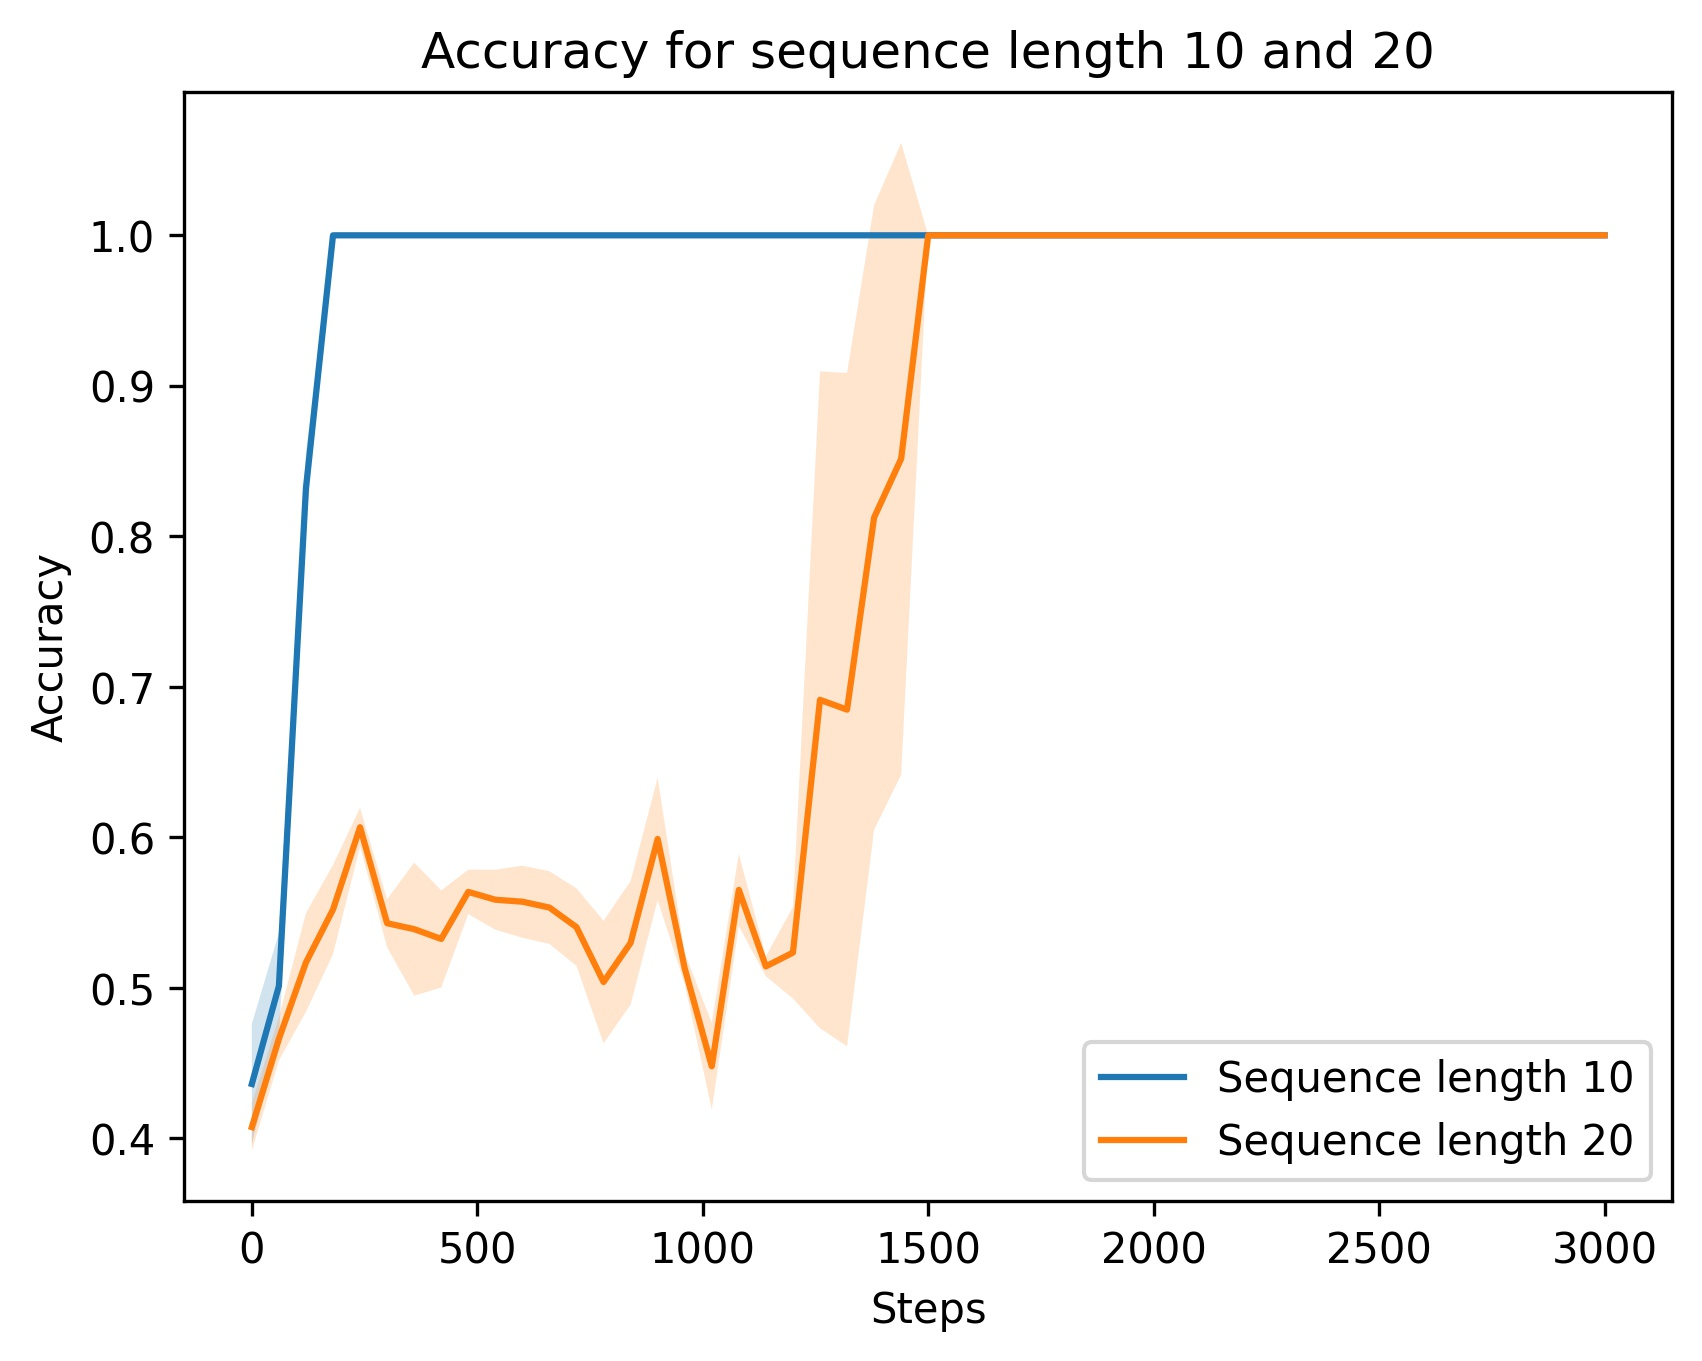
\includegraphics[width=.8\textwidth]{lstm.jpg}}
	\caption{Accuracy of the LSTM on the binary palindrome dataset for $T=10$ and $T = 20$}
	\label{fig:lstm}
\end{figure}
\subsubsection*{Question 1.4}
The peepLSTM model was implemented in PyTorch, using the same hyperparameter settings as before. The results are shown in Figure \ref{fig:peeplstm}. For $T = 20$ the model converges to perfect accuracy already around $500$ steps, which is significantly faster than the original LSTM model. Furthermore, the uncertainty of the accuracy values is much smaller. Apparently, setting the gate values based on the cell states rather than the LSTM outputs is beneficial for the performance of the model on this data set.
\begin{figure}[h]
	\centering
	\subfloat[]{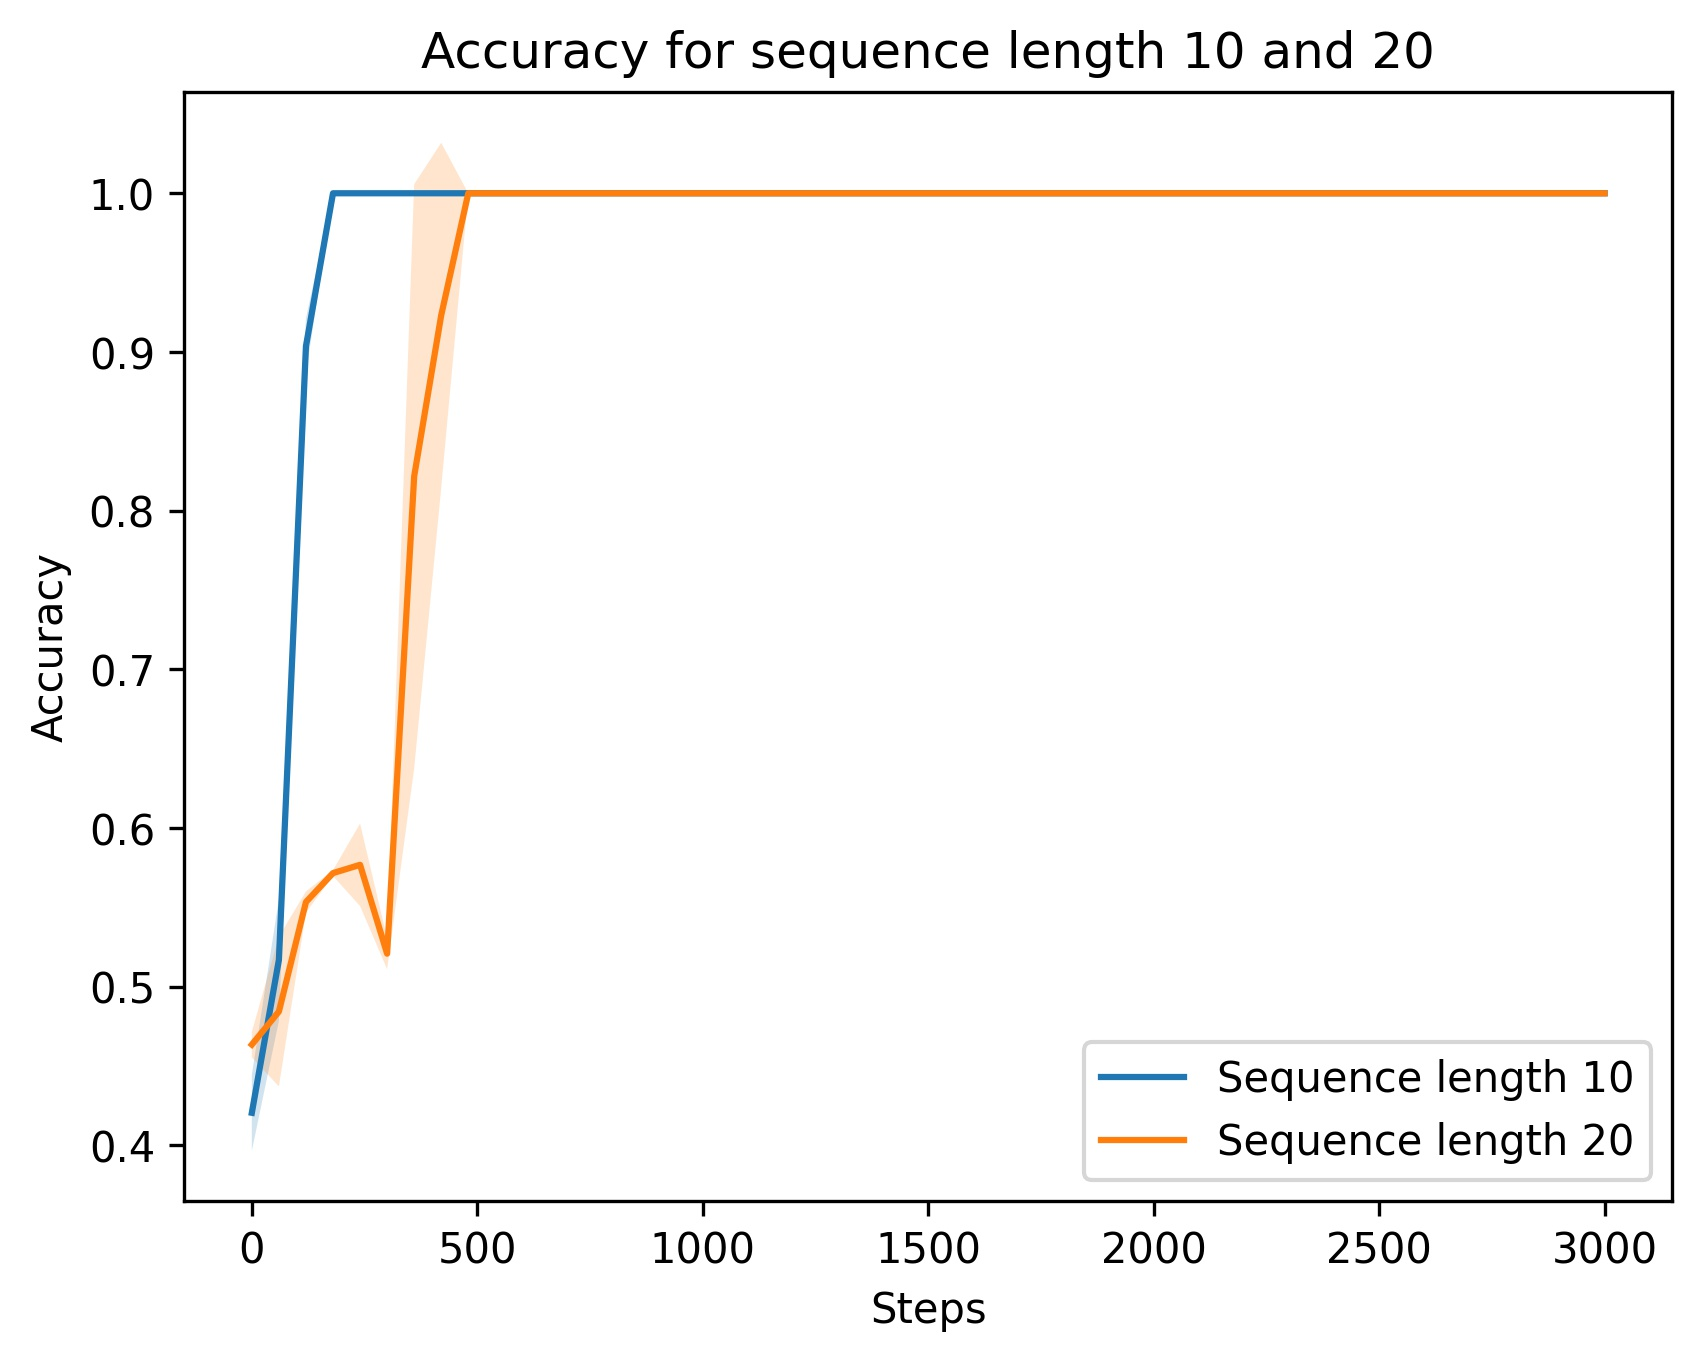
\includegraphics[width=.8\textwidth]{peep_lstm.jpg}}
	\caption{Accuracy of the peepLSTM on the binary palindrome dataset for $T=10$ and $T = 20$}
	\label{fig:peeplstm}
\end{figure}
\section{Recurrent Nets as Generative Model}
\subsubsection*{Question 2.1}
\begin{enumerate}[label = (\alph*)]
	\item The text generation model was implemented using the following hyperparameters:
	\begin{itemize}
		\item Embedding dimension: 64. This value was chosen as it was suggested to use an embedding dimension of $\frac{1}{4}$ of the cell state size.
		\item Batch size: 64. The observed fluctuations in loss and accuracy are quite large for this value, but we still have steady convergence, and we keep the benefit of being able to escape local minima.
	\end{itemize}
	Running the model on Grimms fairy tale dataset for 1500 steps, the loss and accuracy curves are obtained as shown in Figure \ref{fig:texgenacc}:
	\begin{figure}[H]
		\centering
		\subfloat[]{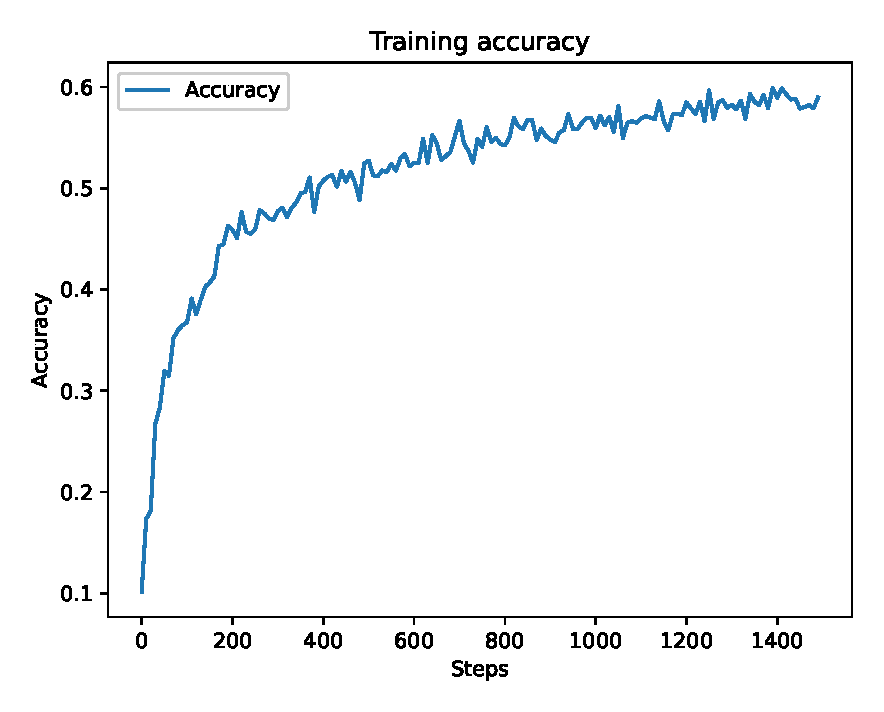
\includegraphics[width=.5\textwidth]{texgenAccuracy.eps}}
		\subfloat[]{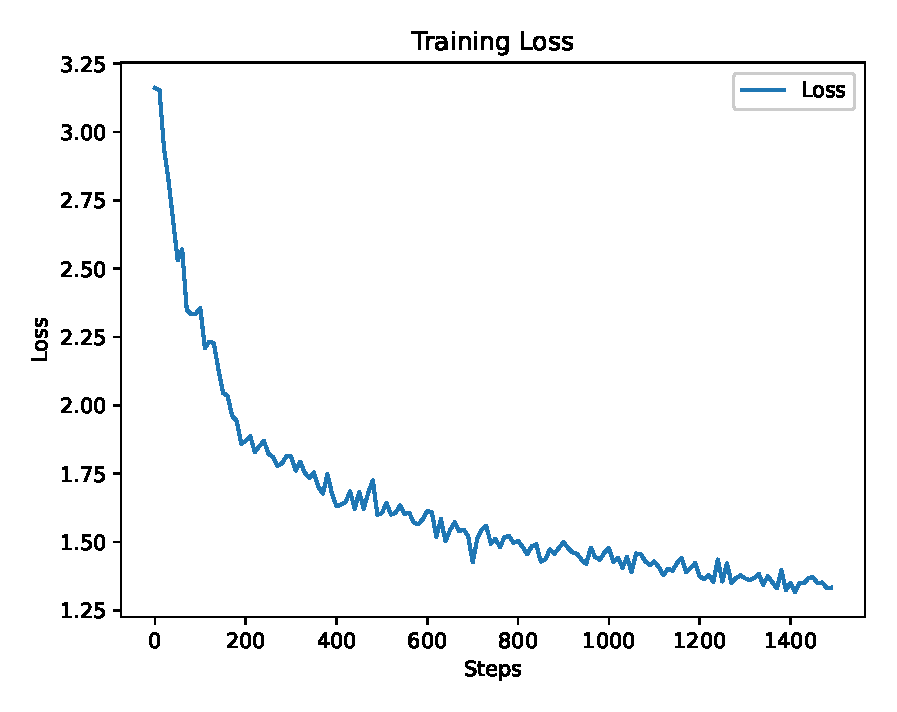
\includegraphics[width=.5\textwidth]{texgenLoss.eps}}
		\caption{Accuracy and loss on the text generation task. The model is trained on the Grimms fairy tale dataset}
		\label{fig:texgenacc}
	\end{figure}
	Notice that the model has not completely converged at 1500 steps. When the model is run for approximately $5000$ steps, it converges to an accuracy of approximately $0.65$. 
	\item Next, the function \texttt{generate\_sequence} was implemented. Below, we list 5 sets of 3 sequences that were generated at $1/3$, $2/3$ and $3/3$ of the $1500$ training iterations. Each set has a different initial character from which the sequences were generated.
	\begin{itemize}
		\item \textbf{Initial character: t}\\
		\textit{1/3}: the forest to the forest to the \\
		\textit{2/3}: the stood the stread to the sto \\
		\textit{3/3}: the world with his father that
		\item \textbf{Initial character: a}\\
		\textit{1/3}: and the wasted the wasted the w \\
		\textit{2/3}: and the bear the bear the bear  \\
		\textit{3/3}: and the sparrow what had not go
		\item \textbf{Initial character: u}\\
		\textit{1/3}: ut the was some to the was some \\
		\textit{2/3}: ut the fire and said: ‘I will s \\
		\textit{3/3}: ut the straw and said, ‘I will 
		\item \textbf{Initial character: v}\\
		\textit{1/3}: ve her her have her her have he \\
		\textit{2/3}: ver the searly and the searly a \\
		\textit{3/3}: ve the stores and said, ‘I will
		\item \textbf{Initial character: g}\\
		\textit{1/3}: g to the stoor and said the sto \\
		\textit{2/3}: g to the wood with the wood wit \\
		\textit{3/3}: g the fire and said, ‘I will go
	\end{itemize}
	From the sequences, it becomes clear that the model is quite vulnerable for getting stuck in loops of words that is has seen with high frequency. Especially prepositions, conjunctions and articles like "in, the, and" are repeated frequently. As the training progresses, longer and more complex dependencies that are frequent in the data become apparent. Notice that the phrase "and said, 'I will" occurs in 3 out of 5 sets of sequences. 
	When we increase the length of generated sequences, we generally observe many repetitions of the same few phrases. This is an artifact of using the argmax to select the next character, because each character will have a unique successor. This makes it easy to get stuck in a loop containing the same characters. 
	\item When the temperature is large, a very large part of the probability density will be assigned to the character with the largest logit, due to the exponential. In other words, the softmax becomes increasingly more like the argmax that was used previously to generate characters. When the temperature is very low, the distribution flattens, and becomes the uniform distribution in the limit of $\tau \to 0$. 
	
	Next, sentences were generated for $\tau \in \{0.5, 1.0, 2.0\}$ using the previous model that was trained to $0.65$ accuracy:
	\begin{itemize}
		\item $\boldsymbol{\tau = 0.5}$: g. Yefuitly; if thought now-Devildres-bacly warm muSif; ‘Blick Stying yon ire! Kul\_Czeby! Is nor pair!’
		‘Heive spife
		rrau;
		but flight a prettil, and te\\
		\item $\boldsymbol{\tau = 1.0}$: great men in his people they did not read
		the ball, he got into the golden cushied. The road behindful of pure
		streamed a white doves danced with you, \\
		\item $\boldsymbol{\tau = 2.0}$: gave his wife sitting and have something and said, ‘I will go to the princesses on the castle
		given her hand, and he got on and the son begged there wa
	\end{itemize}
	For $\tau = 0.5$, the generated words are nonsensical most of the time. Clearly, the distribution is too flat, giving too much probability mass to characters that break the correctness of words. For $\tau = 1.0$, the spelling is correct, but the generated sentences lack syntactic structure. Finally, when $\tau = 2.0$, some syntactic structure can be observed. The span over which this structure is present is small however, which can be attributed to the sequence length that is used. Notice however that the sentences contain few repetitions of phrases, which we observed frequently when using greedy sampling. For generating longer sentences, using the temperature-softmax is clearly the better sampling approach.
\end{enumerate}
\end{document}